\subsection{Attitude Controller}
The attitude controller is designed using a state space representation of the system. This helps handling the coupled angular response of the quadcopter. The chosen states for the system are the three angular positions and the three angular velocities. The input vector consists of the four motor rotational speeds and the output vector consists of the three angles, roll, pitch and yaw. The state, input and output vectors are
%
\begin{flalign}
	\vec{x}(t)&= 
	\begin{bmatrix}
		\phi & \theta & \psi & \dot{\phi} &	\dot{\theta} & \dot{\psi} 
	\end{bmatrix}	\nonumber
	^T,\\
	\vec{y}(t)&= 
	\begin{bmatrix}
		\phi &	\theta & \psi 
	\end{bmatrix}	\nonumber
	^T,\\
	\vec{u}(t)&= 
	\begin{bmatrix}
		\omega_1 & \omega_2 &	\omega_3 &	\omega_4 
	\end{bmatrix}\nonumber	
	^T \ .
\end{flalign}
%
%The vectors above are then used in construction of the state space matrix representation as
%\begin{flalign}
%	\vec{\dot{x}}(t)&=\vec{A} \vec{x}(t) + \vec{B} \vec{u}(t)
%	\label{xDotSS} 
%\end{flalign}
%\vspace{-0.9 cm}
%\begin{flalign}
%	\vec{y}(t)&=\vec{C} \vec{x}(t) + \vec{D} \vec{u}(t)\label{ySS} 
%\end{flalign}
%%
%where $\vec{A}$ is the system matrix, $\vec{B}$ is the input matrix, $\vec{C}$ is the output matrix and $\vec{D}$ is the feedforward matrix.
%
The values for the $\vec{A}$, $\vec{B}$, $\vec{C}$ and $\vec{D}$ matrices in the state space model are obtained from the linearized attitude equations \eqref{eqAngleLin1}, \eqref{eqAngleLin2} and \eqref{eqAngleLin3}, yielding  \fxnote{remove this matrices???}
\vspace{0cm}
\footnotesize{
\begin{align}   
	\vec{A}=
	\begin{bmatrix}
		\ 0 & 0 & 0 & 1 & 0 & 0     \ \ \ \\ 
		\ 0 & 0 & 0 & 0 & 1 & 0     \ \ \ \\ 
		\ 0 & 0 & 0 & 0 & 0 & 1     \ \ \ \\
		\ 0 & 0 & 0 & 0 & 0 & 0     \ \ \ \\ 
		\ 0 & 0 & 0 & 0 & 0 & 0     \ \ \ \\ 
		\ 0 & 0 & 0 & 0 & 0 & 0     \ \ \  
	\end{bmatrix} , \vec{C} =	 
	\begin{bmatrix}
		\ 1 & 0 & 0 & 0 & 0 & 0     \ \ \ \\ 
		\ 0 & 1 & 0 & 0 & 0 & 0     \ \ \ \\ 
		\ 0 & 0 & 1 & 0 & 0 & 0     \ \ \ 
	\end{bmatrix} ,\nonumber
\end{align} 
\vspace{-0.3 cm}
\begin{flalign}
    \vec{B} =
	\begin{bmatrix}
		\ 0 & 0 & 0 & 0      \ \ \ \\ 
		\ 0 & 0 & 0 & 0      \ \ \ \\ 
		\ 0 & 0 & 0 & 0      \ \ \ \\
		\ 0 & \si{-\frac{2  k_{\mathrm{th}} L \overline{\omega}_2}{J_x}} & 0 & \si{\frac{2 k_{\mathrm{th}}  L \overline{\omega}_4}{J_x}}      \ \ \ \\ 
		\ \si{\frac{2 k_{\mathrm{th}} L  \overline{\omega}_1}{J_y}} & 0 & \si{-\frac{2  k_{\mathrm{th}} L \overline{\omega}_3}{J_y}} & 0      \ \ \ \\ 
		\ \frac{2 k_{\mathrm{d}} {\overline{\omega}_1}}{J_z} & - \frac{2 k_{\mathrm{d}} {\overline{\omega}_2}}{J_z} & \frac{2 k_{\mathrm{d}}  {\overline{\omega}_3}}{J_z} & - \frac{2 k_{\mathrm{d}} {\overline{\omega}_4}}{J_z}      		
	\end{bmatrix} \ \ .\nonumber
\end{flalign}
\vspace{0.0 cm}
 }
\normalsize

\noindent Note, that the $\vec{D}$ matrix is a zero matrix.\\
\indent The attitude control is based on a state feedback and an integral term in order to be able to track a given reference and reject input disturbances. As not all states are measured a reduced order observer is implemented to estimate the angular velocities. Due to the separation principle, both subsystems can be designed independently. \cite{ssReference}
\\
\\
\noindent\autoref{AttitudeControlDiagram} shows how these designs are related.
\begin{figure}[H]
    \centering
    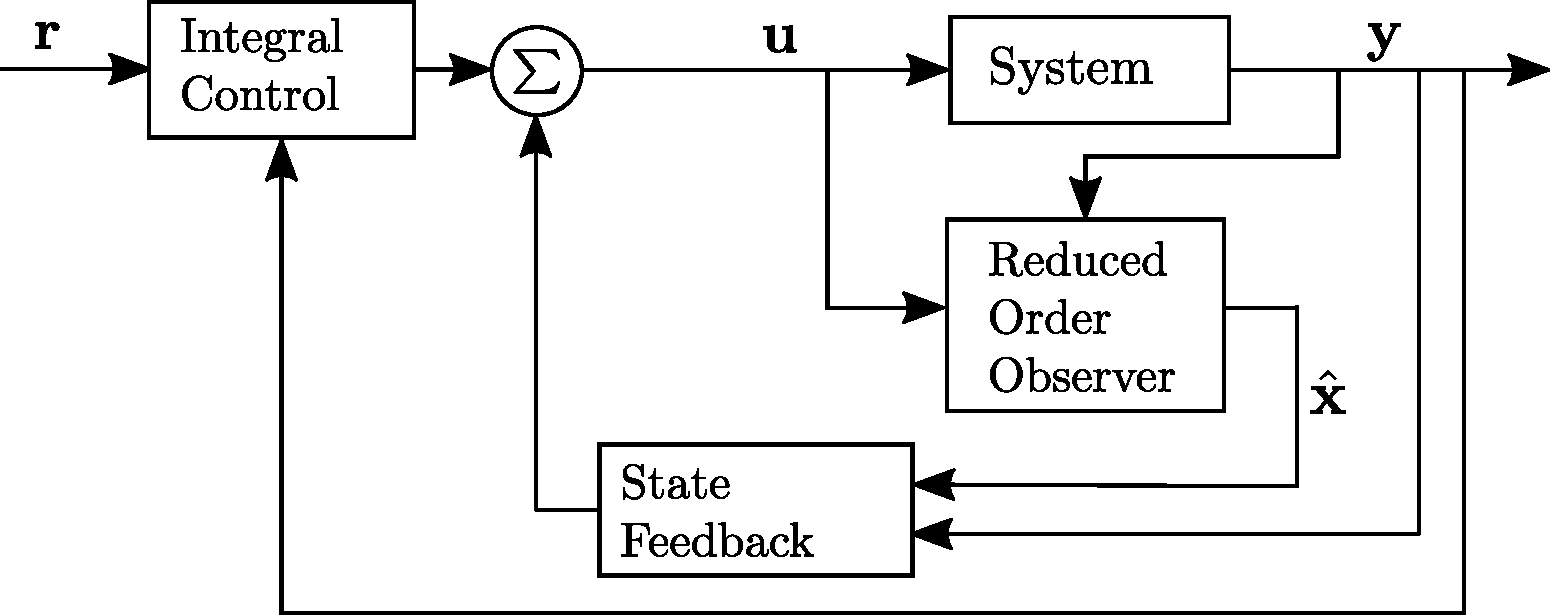
\includegraphics[width=.4\textwidth]{figures/AttitudeControlDiagram}
    \caption{ Control structure for the system, including the state feedback with integral action and the reduced order observer.}
    \label{AttitudeControlDiagram}
\end{figure}

%--------------------- StateFeedback with Integral Control ----------------------------
The design of the state feedback with the integral action is shown in \autoref{fig:DetailedControllerColorDiagram}.
\begin{figure}[H]
    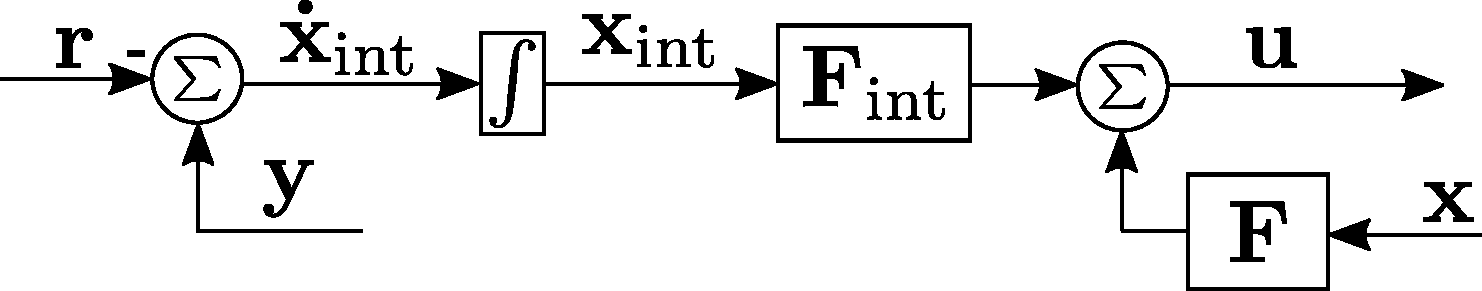
\includegraphics[width=.35\textwidth]{figures/DetailedControllerColorDiagram}
    \centering
    \captionof{figure}{State feedback with integral action in the attitude control structure. $\vec{r}$ is the angular reference vector and $\vec{x}_{\mathrm{int}}$ is the integral states.}
    \label{fig:DetailedControllerColorDiagram}
\end{figure}
Three states, $\vec{x}_{\mathrm{int}}$, are added to the already existing state vector in order to track the two references for $\phi$ and $\theta$ and reject input disturbances in the three angles. This leads to the extended system
%
\vspace{-.2cm}
\begin{flalign} 
\dot{\vec{x}}_\mathrm{e} &= \vec{A}_\mathrm{e} \vec{x}_\mathrm{e} + \vec{B}_\mathrm{e} \vec{u} + 
\begin{bmatrix}
\ \vec{0}     \ \ \ \\ 
\ \vec{-I}     \ \ \  		
\end{bmatrix}
\vec{r}, 
\label{xdotSSExtended}\\ 
\vec{y} &= \vec{C}_\mathrm{e} \vec{x}_\mathrm{e}, 
\label{ySSExtended}
\end{flalign} 
%
where\\
\begin{minipage}{0.45\linewidth}
    \begin{flalign}
    \dot{\vec{x}}_\mathrm{e}= 
    \begin{bmatrix}
    \ \dot{\vec{x}}      \ \  \\ 
    \ \dot{\vec{x}}_{\mathrm{int}}      \ \   		
    \end{bmatrix} , \nonumber
    \end{flalign}
\end{minipage}\hfill
\begin{minipage}{0.45\linewidth}
    \begin{flalign}
    \vec{A}_\mathrm{e}=
    \begin{bmatrix}
    \ \vec{A}  & \vec{0}    \ \  \\ 
    \ \vec{C}  & \vec{0}    \ \   		
    \end{bmatrix} , \nonumber
    \end{flalign}
\end{minipage}   \hfill 

\begin{minipage}{0.45\linewidth}
    \begin{flalign}
        \vec{B}_\mathrm{e}=
        \begin{bmatrix}
            \ \vec{B}    \ \  \\ 
            \ \vec{0}     \ \   		
        \end{bmatrix} ,\nonumber
    \end{flalign}
\end{minipage}\hfill
\begin{minipage}{0.45\linewidth}
    \begin{flalign}
        \vec{C}_\mathrm{e}=
        \begin{bmatrix}
            \ \vec{C}  & \vec{0}  \ \   		
        \end{bmatrix} .\nonumber
    \end{flalign}
\end{minipage}
\\ 
The feedback law is given by 
\begin{flalign} 
	\vec{u} &=\vec{F} \vec{x} + \vec{F}_{\mathrm{int}} \vec{x}_{\mathrm{int}}\ .
	\label{eq:ssControllerAction}
\end{flalign}
The feedback matrix, $\vec{F_{\mathrm{e}}}$ is obtained by using a Linear Quadratic Regulator (LQR) approach together with Bryson's rule. This makes it possible to find the optimal feedback gains while being able to prioritize the different states and set boundaries to the control action.
%
LQR is based on minimizing the following cost function, 
\begin{flalign} 
	J &= \int_{0}^{\infty} \vec{x}^T \vec{Q} \vec{x} + \vec{u}^T \vec{R} \vec{u} dt \ .
	\label{eq:costfunction}
\end{flalign}

The matrices $\vec{Q}$ and $\vec{R}$ must be selected as positive semi-definite and positive definite matrices, respectively. These penalize the error of the different states and inputs of the system. 

These matrices are selected by using Bryson's rule, which defines $\vec{Q}$ and $\vec{R}$ as diagonal matrices whose elements are
\begin{flalign} 
	Q_{ii} &= \frac{1}{\text{maximum acceptable value of }[x^2_i]},\\
	R_{ii} &= \frac{1}{\text{maximum acceptable value of }[u^2_i]}\ .
	\label{eq:weightingmatrices}
\end{flalign}
The values are chosen to ensure stability of the controller while the states converge to the equilibrium point and the references are tracked as fast as possible. This process is performed using the simulation of the model including network effects. 
These values are then used to find the optimal feedback matrices, which minimize the cost function \eqref{eq:costfunction} as 
\begin{flalign} 
	\vec{F}_{\mathrm{e}} &= -\vec{R}^{-1}{\vec{B}_{\mathrm{e}}}^T\vec{P} \ ,
	\label{eq:optimalF}
\end{flalign}
where the matrix $\vec{P}$ is positive definite and its value is found using the Algebraic Riccatti Equation, 
\begin{flalign} 
	\vec{A}_{\mathrm{e}}^T\vec{P}+\vec{P}\vec{A}_{\mathrm{e}}-\vec{P}\vec{B_{\mathrm{e}}}\vec{R}^{-1}\vec{B}_{\mathrm{e}}^T\vec{P}+\vec{Q} &= \vec{0}\ .
	\label{eq:optimalP}
\end{flalign}

Once $\vec{F}_\mathrm{e}$ is obtained, it is split into $\vec{F}$ and $\vec{F}_{\mathrm{int}}$. In this way, the controller is implemented as shown in \autoref{fig:DetailedControllerColorDiagram}.\\
%--------------------- Reduced-Order Observer ----------------------------

The reduced observer estimates the angular velocities by means of the system input and output. With this approach, the first three states, $\vec{x}_{1:3}$, are equal to the outputs, $\vec{y}$, whereas the other three states, $\vec{x}_{4:6}$, are estimated as $\hat{\vec{x}}_{4:6}$. 

The observer is designed by finding the matrix $\vec{L}_{\mathrm{obs}}$ such that the eigenvalues of the matrix $\vec{A}_{22}+\vec{L}_{\mathrm{obs}}\vec{A}_{12}$ have negative real part. This makes the estimate converge to the true angular velocity \cite{ssReference}. This is performed by splitting the original system matrices into the submatrices\\
%
\begin{minipage}{0.45\linewidth}
    \begin{flalign}
    \vec{A}=
    \begin{bmatrix}
    \ \vec{A}_{11}  & \vec{A}_{12}    \ \ \ \\ 
    \ \vec{A}_{21}  & \vec{A}_{22}    \ \ \  		
    \end{bmatrix}, \nonumber
    \end{flalign}
\end{minipage}   \hfill 
\begin{minipage}{0.45\linewidth}
    \begin{flalign}
    \vec{B}=
    \begin{bmatrix}
    \ \vec{B}_1    \ \ \ \\ 
    \ \vec{B}_2     \ \ \  		
    \end{bmatrix} \ . \nonumber
    \end{flalign}
\end{minipage}\\
\normalsize

With the observer matrix, the observer equation is derived, see \eqref{eq:eqobservertheorem}. This ensures an estimate $\hat{\vec{x}}_{4:6}$ which converges to $\vec{x}_{4:6}$ at a rate given by the chosen observer poles.
\small{
\begin{flalign}
\vec{\dot{\hat{x}}_{4:6}} + \vec{L}_{\mathrm{obs}}\dot{y} &= (\vec{A}_{22}+\vec{L}_{\mathrm{obs}}\vec{A}_{12})\vec{\hat{x}}_{4:6}\label{eq:eqobservertheorem} \\&+(\vec{A}_{21}+\vec{L}_{\mathrm{obs}}\vec{A}_{11})\vec{y}+(\vec{B}_2+\vec{L}_{\mathrm{obs}}\vec{B}_1)\vec{u}\nonumber
%    \vec{\hat{\dot{x}}}_{4:6} &= \vec{A}_{21}\vec{y} + \vec{A}_{22}\vec{\hat{x}}_{4:6} + \vec{B_2}\vec{u} + \vec{L}_{\mathrm{obs}}\vec{(A}_{12}\vec{\hat{x}}_{4:6} - \vec{A}_{21}\vec{x}_{4:6})
\end{flalign}
\normalsize

The estimation of $\vec{x}_{4:6}$ is implemented as shown in \autoref{fig:observerDiagram}.

\begin{figure}[H]
    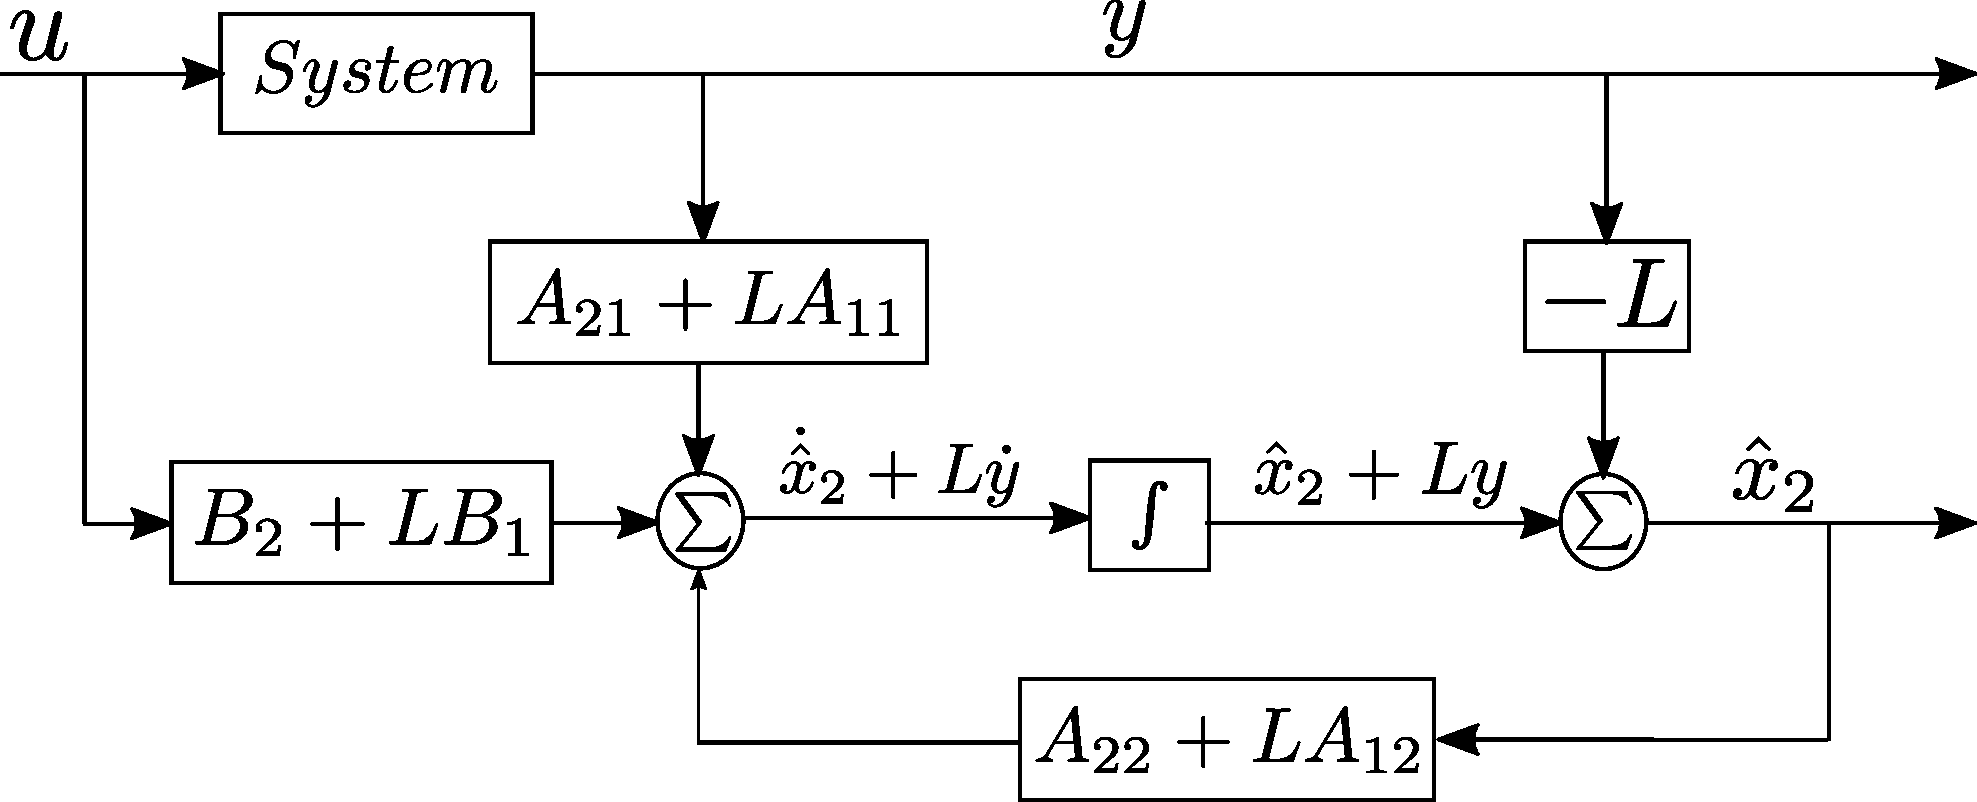
\includegraphics[width=.45\textwidth]{figures/observerDiagram}
    \centering
    \captionsetup{justification=centering}
    \captionof{figure}{Detailed diagram of the reduced order observer illustrating its implementation.}
    \label{fig:observerDiagram}
\end{figure}